\documentclass[%
  reprint,
  twocolumn,
 %superscriptaddress,
 %groupedaddress,
 %unsortedaddress,
 %runinaddress,
 %frontmatterverbose,
 % preprint,
 showpacs,
 showkeys,
 preprintnumbers,
 %nofootinbib,
 %nobibnotes,
 %bibnotes,
 amsmath,amssymb,
 aps,
 % prl,
 pra,
 % prb,
 % rmp,
 %prstab,
 %prstper,
  longbibliography,
 %floatfix,
 %lengthcheck,%
 ]{revtex4-1}

%\usepackage{cdmtcs-pdf}

\usepackage[dvipsnames]{xcolor}

\usepackage{mathptmx}% http://ctan.org/pkg/mathptmx

\usepackage{amssymb,amsthm,amsmath}

\usepackage{tikz}
\usetikzlibrary{calc,decorations.pathreplacing,decorations.markings,positioning,shapes}

\usepackage[breaklinks=true,colorlinks=true,anchorcolor=blue,citecolor=blue,filecolor=blue,menucolor=blue,pagecolor=blue,urlcolor=blue,linkcolor=blue]{hyperref}
\usepackage{graphicx}% Include figure files
\usepackage{url}


\begin{document}

\title{(Non)contextual coloring of orthogonality hypergraphs}

\author{Mohammad Hadi Shekarriz}

\author{Karl Svozil}
\email{svozil@tuwien.ac.at}
\homepage{http://tph.tuwien.ac.at/~svozil}

\affiliation{Institute for Theoretical Physics,
Vienna  University of Technology,
Wiedner Hauptstrasse 8-10/136,
1040 Vienna,  Austria}


\date{\today}

\begin{abstract}
Chromatic constructions on orthogonality hypergraphs which are classical set representable or have a faithful orthogonal representation are discussed. The latter ones have a quantum mechanical realization as a context or maximal observable.
\end{abstract}

\keywords{Quantum mechanics, Gleason theorem, Kochen-Specker theorem, Born rule, gadget graphs}
\pacs{03.65.Ca, 02.50.-r, 02.10.-v, 03.65.Aa, 03.67.Ac, 03.65.Ud}

\maketitle


% MDPI  \PassOptionsToPackage{dvipsnames}{xcolor}
% MDPI  \documentclass[entropy,article,submit,oneauthor,pdftex]{Definitions/mdpi}
% MDPI
% MDPI
% MDPI  %%%%%%%%%%%%%%%%%%%%%%%%%%%%%%%%%%%%%%%%%%%%%%%%%%%%%%%%%%%%%%%%%%%%%%%%%%%%%%%%%%%%%%%%%%%%%%%%%%%%%%%%%%%%%%%%%%%%%%%%%%%%%%%%%%%%%%%%%%%%%%%%
% MDPI  \usepackage{graphicx}% Include figure files
% MDPI
% MDPI  \usepackage{amssymb}
% MDPI
% MDPI  \usepackage{tikz}
% MDPI  \usetikzlibrary{calc,decorations.pathreplacing,decorations.markings,positioning,shapes}
% MDPI
% MDPI  \newcommand{\ruledtabular}{\hline \hline}
% MDPI
% MDPI  %%%%%%%%%%%%%%%%%%%%%%%%%%%%%%%%%%%%%%%%%%%%%%%%%%%%%%%%%%%%%%%%%%%%%%%%%%%%%%%%%%%%%%%%%%%%%%%%%%%%%%%%%%%%%%%%%%%%%%%%%%%%%%%%%%%%%%%%%%%%%%%%
% MDPI
% MDPI
% MDPI
% MDPI  \firstpage{1}
% MDPI  \makeatletter
% MDPI  \setcounter{page}{\@firstpage}
% MDPI  \makeatother
% MDPI  \pubvolume{xx}
% MDPI  \issuenum{1}
% MDPI  \articlenumber{5}
% MDPI  \pubyear{2019}
% MDPI  \copyrightyear{2019}
% MDPI  %\externaleditor{Academic Editor: name}
% MDPI  %\history{Received: date; Accepted: date; Published: date}
% MDPI  %\updates{yes} % If there is an update available, un-comment this line
% MDPI
% MDPI  %% MDPI internal command: uncomment if new journal that already uses continuous page numbers
% MDPI  %\continuouspages{yes}
% MDPI
% MDPI  %------------------------------------------------------------------
% MDPI  % The following line should be uncommented if the LaTeX file is uploaded to arXiv.org
% MDPI  %\pdfoutput=1
% MDPI
% MDPI  %=================================================================
% MDPI  % Add packages and commands here. The following packages are loaded in our class file: fontenc, calc, indentfirst, fancyhdr, graphicx, lastpage, ifthen, lineno, float, amsmath, setspace, enumitem, mathpazo, booktabs, titlesec, etoolbox, amsthm, hyphenat, natbib, hyperref, footmisc, geometry, caption, url, mdframed, tabto, soul, multirow, microtype, tikz
% MDPI
% MDPI  %=================================================================
% MDPI  %% Please use the following mathematics environments: Theorem, Lemma, Corollary, Proposition, Characterization, Property, Problem, Example, ExamplesandDefinitions, Hypothesis, Remark, Definition, Notation, Assumption
% MDPI  %% For proofs, please use the proof environment (the amsthm package is loaded by the MDPI class).
% MDPI
% MDPI  %=================================================================
% MDPI  % Full title of the paper (Capitalized)
% MDPI  \Title{Classical predictions for intertwined quantum observables are contingent and thus inconclusive}
% MDPI  %\thanks{This is a largely revised and extended version of a paper which has been published somewhat hidden in Section~12.9 of my recent book on (A)Causality~\cite{svozil-pac}.}
% MDPI
% MDPI  % Author Orchid ID: enter ID or remove command
% MDPI  \newcommand{\orcidauthorA}{0000-0001-6554-2802} % Add \orcidA{} behind the author's name
% MDPI
% MDPI  % Authors, for the paper (add full first names)
% MDPI  \Author{Karl Svozil $^{1}$*}
% MDPI
% MDPI  % Authors, for metadata in PDF
% MDPI  \AuthorNames{Karl Svozil}
% MDPI
% MDPI  % Affiliations / Addresses (Add [1] after \address if there is only one affiliation.)
% MDPI  \address{$^{1}$ \quad Institute for Theoretical Physics, Vienna University of Technology, Wiedner Hauptstrasse 8-10/136, A-1040 Vienna, Austria, EU; svozil@tuwien.ac.at}
% MDPI
% MDPI  % Contact information of the corresponding author
% MDPI  %\corres{Correspondence: e-mail@e-mail.com; Tel.: (optional; include country code; if there are multiple corresponding authors, add author initials) +xx-xxxx-xxx-xxxx (F.L.)}
% MDPI
% MDPI  % Current address and/or shared authorship
% MDPI  %\firstnote{Current address: Affiliation 3}
% MDPI  %\secondnote{These authors contributed equally to this work.}
% MDPI  % The commands \thirdnote{} till \eighthnote{} are available for further notes
% MDPI
% MDPI  %\simplesumm{} % Simple summary
% MDPI
% MDPI  %\conference{} % An extended version of a conference paper
% MDPI
% MDPI  % Abstract (Do not insert blank lines, i.e. \\)
% MDPI  \abstract{Classical evaluations of configurations of intertwined quantum contexts induce relations, such as true-implies-false, true-implies-true~\cite{2018-minimalYIYS}, but also nonseparability among the input and output terminals. When combined, these exploitable configurations (aka gadgets) deliver the strongest form of classical value indefiniteness. However, the choice of the respective configuration among all such collections, and thus the relation of its terminals, remains arbitrary and cannot be motivated by some superselection principle inherent to quantum or classical physics.}
% MDPI  % Keywords
% MDPI  \keyword{Quantum mechanics, Gleason theorem, Kochen-Specker theorem, Born rule, gadget graphs}
% MDPI
% MDPI  % The fields PACS, MSC, and JEL may be left empty or commented out if not applicable
% MDPI  \PACS{03.65.Ca, 02.50.-r, 02.10.-v, 03.65.Aa, 03.67.Ac, 03.65.Ud}
% MDPI  %\MSC{}
% MDPI  %\JEL{}
% MDPI
% MDPI  %%%%%%%%%%%%%%%%%%%%%%%%%%%%%%%%%%%%%%%%%%
% MDPI  % Only for the journal Diversity
% MDPI  %\LSID{\url{http://}}
% MDPI
% MDPI  %%%%%%%%%%%%%%%%%%%%%%%%%%%%%%%%%%%%%%%%%%
% MDPI  % Only for the journal Applied Sciences:
% MDPI  %\featuredapplication{Authors are encouraged to provide a concise description of the specific application or a potential application of the work. This section is not mandatory.}
% MDPI  %%%%%%%%%%%%%%%%%%%%%%%%%%%%%%%%%%%%%%%%%%
% MDPI
% MDPI  %%%%%%%%%%%%%%%%%%%%%%%%%%%%%%%%%%%%%%%%%%
% MDPI  % Only for the journal Data:
% MDPI  %\dataset{DOI number or link to the deposited data set in cases where the data set is published or set to be published separately. If the data set is submitted and will be published as a supplement to this paper in the journal Data, this field will be filled by the editors of the journal. In this case, please make sure to submit the data set as a supplement when entering your manuscript into our manuscript editorial system.}
% MDPI
% MDPI  %\datasetlicense{license under which the data set is made available (CC0, CC-BY, CC-BY-SA, CC-BY-NC, etc.)}
% MDPI
% MDPI  %%%%%%%%%%%%%%%%%%%%%%%%%%%%%%%%%%%%%%%%%%
% MDPI  % Only for the journal Toxins
% MDPI  %\keycontribution{The breakthroughs or highlights of the manuscript. Authors can write one or two sentences to describe the most important part of the paper.}
% MDPI
% MDPI  %\setcounter{secnumdepth}{4}
% MDPI  %%%%%%%%%%%%%%%%%%%%%%%%%%%%%%%%%%%%%%%%%%
% MDPI \begin{document}

\setcounter{MaxMatrixCols}{20}

\section{Nomenclature}

In what follows w eshall use the following terms will be used synonymuously:
context, block, (Boolean) subalgebra, (maximal) clique, complete graph.

Greechie has suggested~\cite{greechie:71} to (amendmends are indicated by square brackets ``[$\ldots$]'')
\begin{quote}
[$\ldots$]
present [$\ldots$] lattices as unions of [contexts]
intertwined or pasted together in some fashion
[$\ldots$]
by replacing, for example, the $2^n$ elements in the Hasse diagram of the power set
of an $n$-element set with the [context aka] complete graph [$K_n$] on $n$ elements.
The reduction in numbers of elements is considerable but the number of remaining ``links''
or ``lines'' is still too cumbersome for our purposes.
We replace the [context aka] complete graph on $n$ elements by a single smooth curve (usually a straight line)
containing $n$ distinguished points. Thus we replace $n(n + 1)/2$ ``links'' with a single smooth curve.
This representation is propitious and uncomplicated provided that
the intersection of any pair of blocks contains at most one atom.
\end{quote}
In what follows we shall refer to such a hypergraph representation as {Greechie diagram}~\cite{kalmbach-83}.

We shall concentrate on Greechie diagrams which are pasting~\cite{Greechie1968} constructions~\cite[Chapter~2]{greechie-66-PhD}
of a homogenuous  single type
of contexts $K_n$
where the clique number $n$ is fixed.
In what follows we shall refer to the Greechie diagrammatical representation of
such, possibly intertwined, collection of blocks, as {\em hypergraph}.

A hypergraph coloring is a uniform coloring which associates $n$ mutually different colors
to every atomic element of each context.
That is, the $n$ distinguished points of any single smooth curve in the hypergraph have $n$ different colors.
The coloring is noncontextual; that is, the coloring of atomic elements common to two or more contexts (intertwining there)
is independent of the context.
In requirng uniformity we shall implicitly also exclude partial colorings~\cite{Abbott:2010uq,PhysRevA.89.032109,2015-AnalyticKS}
whers partiality is understood as allowing for undefinedness in the sense of Kleene~\cite{Kleene1936}.

The chromatic number $m$ of a hypergraph is the minimal number of mutually different colors in any coloring of this hypergraph.
It is bound from below by the clique number $n$.
If these numbers are the same, that is, if $n=m$, then one could obtain two-valued measures from colorings by ``projecting''
one of the colors into the value 1, and all the other $m-1$ colors into the value 0~\cite{godsil-zaks,meyer:99,havlicek-2000}.


Finite examples for which the chromatic number exceeds the clique number, that is, $m>n$,
are the logical structures involved in proofs of the Kochen-Specker theorem.
Explicit constructions are, for instance,
$\Gamma_2$ of Ref.~\cite{kochen1},
as well as the configurations enumerated in
Fig.~9 of~\cite{svozil-tkadlec},
Fig.~1--3 of~\cite{tkadlec-00},
Ref.~\cite{cabello-96},
as well as Table~I, Fig.~2 of Ref.~\cite{2015-AnalyticKS},
among numerous others
which have a faithful orthogonal representation~\cite{lovasz-79,lovasz-89,Portillo-2015}
in ``small dimensions'' greater than two.





\section{Chromatic construction from two-valued states}


Conjecture: the following statements are equivalent:

\begin{itemize}
\item[(i)]
The chromatic number of the hypergraph equals the clique number $n$; that is, the associated graph is colorable by $n$ distinct colors.
\item[(ii)]
The set of two-valued states contains $n$ states which correspond
to a partitioning of all elements of the partition logic;
the equivalence relation defined by each one of these $n$ states evaluating to $1$ on some element of every context.
That is, those $n$ states are $1$ on different atoms of every context.
\end{itemize}

Conjecture: the following statements are equivalent:

\begin{itemize}
\item[(i)]
Whenever the chromatic number of the hypergraph equals the clique number $n$,
then this  collection of (intertwined) contexts possesses a separating set of two-valued states.
This means that it is homomorphically embeddable into a Boolean algebra~\cite[Theorem~0]{kochen1},
which in turn means that it is set representable as a partition logic~\cite{schaller-92}.
\item[(ii)]
There exists a (nonunique) ``canonical construction'' of a partition logic
from its set of two-valued states~\cite{svozil-2001-eua} facilitating such a coloring with $n$ colors.
\end{itemize}




\section{Babylonian evidence~\cite{neugeb} by anecdotal (counter-)examples}

A (nonunique) coloring can (at least for some hypergraphs) be effectively constructed as follows:

\begin{enumerate}
\item[(1)] Choose two arbitrary contexts
$C_1 =\{a_1,\ldots ,a_n\}$ and $C_2=\{b_1,\ldots ,b_n\}$ of the logic (represented by the respective hypergraph).

\item[(2)]
In $C_1$ choose an arbitrary atom, say $a_i$; and identify the first color $\chi_1$
with any single one non-vanishing (on $a_i$) two-valued state $s_j(a_i) =1$ of choice.
Moreover, assign $a_i$  this first color $\chi_1$.

\item[(3)] Associate within $C_2$ the unique single atom $b_j$ for which $s_j$ does not vanish
-- that is, $s_j(b_j)=1$ -- and assign $b_j$  the first color $\chi_1$.

\item[(4)] Discard all two-valued states $s$ which:

\begin{enumerate}
\item[(4.1)] either do not vanish on $a_i$; that is, only states $s \in S$ remain with $s(a_i)=0$.
[By the assumption of separability the set of remaining states is not empty (this is crucial).]

\item[(4.2)] or do not vanish on any atom $e_{kl}$ on each context $C_k$ (there will be one atom $e_{kl}$ per context $C_k$)
for which $s_j(e_{kl})=1$; that is, only states $s \in S$ remain with $s(e_{kl})=0$ for all contexts labelled by $k$.
[Note: (4.1) is a subcase of (4.2), so (4.1) is redundant and only (4.2) needs to be mentioned.]

\end{enumerate}
\item[(5)] Then repeat (2) and  choose a second atom $a_{i'}$ from $C_1$;
and associate the second color $\chi_2$ with any single one non-vanishing (on $a_{i'}$)
remaining two-valued state $s_{j'}(a_{i'}) =1$ of choice.

\item[(6)] Then repeat (3) and  associate within $C_2$ those singe atom $b_{j'}$
for which $s_{j'}$ does not vanish -- that is, $s_{j'}(b_{j'})=1$ -- and color it with the second color $\chi_2$.

By construction (elimination of all two-valued states which do not vanish on all previously colored atoms)
this atom $b_{j'}$ must be different from $b_j$ (both $b_j$ as well as $b_{j'}$ are in $C_2$).

\item[(7)] Then repeat (4).

\item[(8)] Repeat (2)-(4) until all atoms of the first context $C_1$ are covered.

\end{enumerate}
This completes the coloring of allatoms of the hypergraph, and thus the direct proof.



\subsection{Examples}
\subsubsection{Triangle logic}

The coloring procedure of the triangle hypergraph is depicted in Fig.~\ref{2020-f-chroma-triangle3}.
Consider the set of all four two-valued states on the six atoms which can be tabulated by a
(compactified) Travis~\cite{travis-mt-62} matrix~\cite{greechie-66-PhD} $T_{ij}$
whose rows indicate the
$i$th state $s_i$ and whose columns
indicate the atoms $a_j$, respectively; that is, $T_{ij}=s_i(a_j)$:
\begin{equation}
T_{ij}=\begin{pmatrix}
{\color{red}1}&{\color{red}0}&{\color{red}0}&{\color{red}1}&{\color{red}0}&{\color{red}0}\\
{\color{blue}0}&{\color{blue}0}&{\color{blue}1}&{\color{blue}0}&{\color{blue}0}&{\color{blue}1}\\
{\color{green}0}&{\color{green}1}&{\color{green}0}&{\color{green}0}&{\color{green}1}&{\color{green}0}\\
0&1&0&1&0&1
\end{pmatrix}
.
\end{equation}
It is not too dificult to see that the first three measures, represented by the first three row vectors of the
Travis matrix, add up to
$
\begin{pmatrix}
1,1,1,1,1,1
\end{pmatrix}
$. They can thus be taken as the basis of a coloring.

\begin{figure}
\begin{center}
\begin{tabular}{ c c c c }
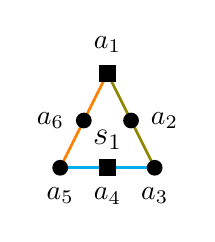
\begin{tikzpicture}  [scale=0.6]

\tikzstyle{every path}=[line width=1pt]

\newdimen\ms
\ms=0.1cm
\tikzstyle{s1}=[color=black,fill,rectangle,inner sep=3]
\tikzstyle{c1}=[color=black,fill,circle,inner sep={\ms/8},minimum size=2*\ms]

% Define positions of all observables


\coordinate (a1) at  (1,2);
\coordinate (a2) at (1.5,1);
\coordinate (a3) at (2,0);
\coordinate (a4) at (1,0);
\coordinate (a5) at (0,0);
\coordinate (a6) at (0.5,1);
\coordinate (c) at (1,0.6);

% draw contexts

\draw [color=olive] (a1) -- (a3);
\draw [color=cyan] (a3) -- (a5);
\draw [color=orange] (a5) -- (a1);


% draw atoms

\draw (a1) coordinate[s1,label=above:$a_1$];
\draw (a2) coordinate[c1,label=right:$a_2$];
\draw (a3) coordinate[c1,label=below:$a_3$];
\draw (a4) coordinate[s1,label=below:$a_4$];
\draw (a5) coordinate[c1,label=below:$a_5$];
\draw (a6) coordinate[c1,label=left:$a_6$];
\node at (c) {\large $s_1$};

\end{tikzpicture}
&
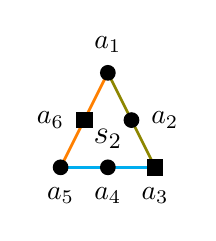
\begin{tikzpicture}  [scale=0.6]

\tikzstyle{every path}=[line width=1pt]

\newdimen\ms
\ms=0.1cm
\tikzstyle{s1}=[color=black,fill,rectangle,inner sep=3]
\tikzstyle{c1}=[color=black,fill,circle,inner sep={\ms/8},minimum size=2*\ms]

% Define positions of all observables


\coordinate (a1) at  (1,2);
\coordinate (a2) at (1.5,1);
\coordinate (a3) at (2,0);
\coordinate (a4) at (1,0);
\coordinate (a5) at (0,0);
\coordinate (a6) at (0.5,1);
\coordinate (c) at (1,0.6);

% draw contexts

\draw [color=olive] (a1) -- (a3);
\draw [color=cyan] (a3) -- (a5);
\draw [color=orange] (a5) -- (a1);


% draw atoms

\draw (a1) coordinate[c1,label=above:$a_1$];
\draw (a2) coordinate[c1,label=right:$a_2$];
\draw (a3) coordinate[s1,label=below:$a_3$];
\draw (a4) coordinate[c1,label=below:$a_4$];
\draw (a5) coordinate[c1,label=below:$a_5$];
\draw (a6) coordinate[s1,label=left:$a_6$];
\coordinate (c) at (1,0.6);
\node at (c) {\large $s_2$};

\end{tikzpicture}
&
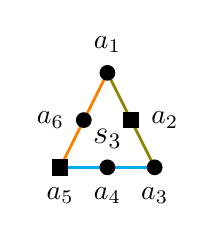
\begin{tikzpicture}  [scale=0.6]

\tikzstyle{every path}=[line width=1pt]

\newdimen\ms
\ms=0.1cm
\tikzstyle{s1}=[color=black,fill,rectangle,inner sep=3]
\tikzstyle{c1}=[color=black,fill,circle,inner sep={\ms/8},minimum size=2*\ms]

% Define positions of all observables


\coordinate (a1) at  (1,2);
\coordinate (a2) at (1.5,1);
\coordinate (a3) at (2,0);
\coordinate (a4) at (1,0);
\coordinate (a5) at (0,0);
\coordinate (a6) at (0.5,1);
\coordinate (c) at (1,0.6);

% draw contexts

\draw [color=olive] (a1) -- (a3);
\draw [color=cyan] (a3) -- (a5);
\draw [color=orange] (a5) -- (a1);


% draw atoms

\draw (a1) coordinate[c1,label=above:$a_1$];
\draw (a2) coordinate[s1,label=right:$a_2$];
\draw (a3) coordinate[c1,label=below:$a_3$];
\draw (a4) coordinate[c1,label=below:$a_4$];
\draw (a5) coordinate[s1,label=below:$a_5$];
\draw (a6) coordinate[c1,label=left:$a_6$];
\node at (c) {\large $s_3$};

\end{tikzpicture}
&
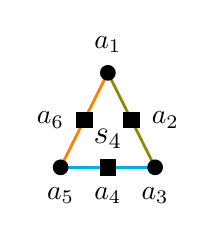
\begin{tikzpicture}  [scale=0.6]

\tikzstyle{every path}=[line width=1pt]

\newdimen\ms
\ms=0.1cm
\tikzstyle{s1}=[color=black,fill,rectangle,inner sep=3]
\tikzstyle{c1}=[color=black,fill,circle,inner sep={\ms/8},minimum size=2*\ms]

% Define positions of all observables


\coordinate (a1) at  (1,2);
\coordinate (a2) at (1.5,1);
\coordinate (a3) at (2,0);
\coordinate (a4) at (1,0);
\coordinate (a5) at (0,0);
\coordinate (a6) at (0.5,1);
\coordinate (c) at (1,0.6);

% draw contexts

\draw [color=olive] (a1) -- (a3);
\draw [color=cyan] (a3) -- (a5);
\draw [color=orange] (a5) -- (a1);


% draw atoms

\draw (a1) coordinate[c1,label=above:$a_1$];
\draw (a2) coordinate[s1,label=right:$a_2$];
\draw (a3) coordinate[c1,label=below:$a_3$];
\draw (a4) coordinate[s1,label=below:$a_4$];
\draw (a5) coordinate[c1,label=below:$a_5$];
\draw (a6) coordinate[s1,label=left:$a_6$];
\node at (c) {\large $s_4$};

\end{tikzpicture}
%
\\
%
(a)&(b)&(c)&(d)\\
%
\end{tabular}
%
\\
%
\begin{tabular}{ c c }
%
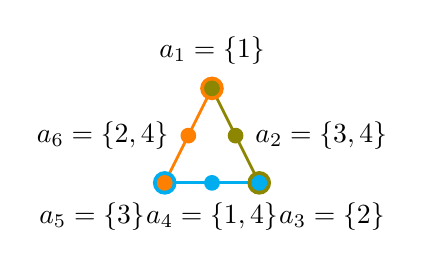
\begin{tikzpicture}  [scale=0.6]

\tikzstyle{every path}=[line width=1pt]

\newdimen\ms
\ms=0.1cm
\tikzstyle{c2}=[circle,inner sep={\ms/8},minimum size=3*\ms]
\tikzstyle{c1}=[circle,inner sep={\ms/8},minimum size=2*\ms]

% Define positions of all observables


\coordinate (a1) at  (1,2);
\coordinate (a2) at (1.5,1);
\coordinate (a3) at (2,0);
\coordinate (a4) at (1,0);
\coordinate (a5) at (0,0);
\coordinate (a6) at (0.5,1);

% draw contexts

\draw [color=olive] (a1) -- (a3);
\draw [color=cyan] (a3) -- (a5);
\draw [color=orange] (a5) -- (a1);


% draw atoms

\draw (a1) coordinate[c2,fill=orange,label=above:${a_1=\{1\}}$];
\draw (a1) coordinate[c1,fill=olive];

\draw (a2) coordinate[c1,fill=olive,label=right:${a_2=\{3,4\}}$];

\draw (a3) coordinate[c2,fill=olive,label=below right:${a_3=\{2\}}$];
\draw (a3) coordinate[c1,fill=cyan];

\draw (a4) coordinate[c1,fill=cyan,label=below:${a_4=\{1,4\}}$];

\draw (a5) coordinate[c2,fill=cyan,label=below left:${a_5=\{3\}}$];
\draw (a5) coordinate[c1,fill=orange];

\draw (a6) coordinate[c1,fill=orange,label=left:${a_6=\{2,4\}}$];

\end{tikzpicture}
&
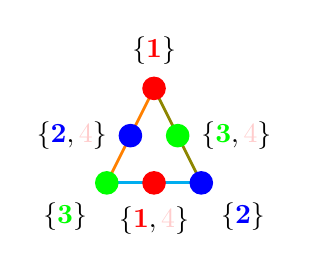
\begin{tikzpicture}  [scale=0.6]

\tikzstyle{every path}=[line width=1pt]

\newdimen\ms
\ms=0.1cm
\tikzstyle{c2}=[circle,inner sep={\ms/8},minimum size=3*\ms]
\tikzstyle{c1}=[circle,inner sep={\ms/8},minimum size=2*\ms]

% Define positions of all observables


\coordinate (a1) at  (1,2);
\coordinate (a2) at (1.5,1);
\coordinate (a3) at (2,0);
\coordinate (a4) at (1,0);
\coordinate (a5) at (0,0);
\coordinate (a6) at (0.5,1);

% draw contexts

\draw [color=olive] (a1) -- (a3);
\draw [color=cyan] (a3) -- (a5);
\draw [color=orange] (a5) -- (a1);


% draw atoms

\draw (a1) coordinate[c2,fill=red,label=above:${\{{\color{red} \bf 1}\}}$];

\draw (a2) coordinate[c2,fill=green,label=right:${\{{\color{green} \bf 3},{\color{red!20!white} 4}\}}$];

\draw (a3) coordinate[c2,fill=blue,label=below right:${\{{\color{blue} \bf 2}\}}$];


\draw (a4) coordinate[c2,fill=red,label=below:${\{{\color{red} \bf 1},{\color{red!20!white} 4}\}}$];

\draw (a5) coordinate[c2,fill=green,label=below left:${\{{\color{green} \bf 3}\}}$];


\draw (a6) coordinate[c2,fill=blue,label=left:${\{{\color{blue} \bf 2},{\color{red!20!white} 4}\}}$];

\end{tikzpicture}
%
\\
%
(e)&(f)
\end{tabular}
\end{center}
\caption{\label{2020-f-chroma-triangle3}
One (nonunique) coloring~(f) construction of
the triangle hypergraph of the logic: first compose a (nonunique)
canonical partition logic~(e) from enumerating the set of all 4 two-valued states depicted in (a)--(d).
Then chose the context $\{a_1,a_2,a_3\}$, and from this context choose the atom $a_1=\{1\}$.
Now identify the first color (red) with the index 1, thereby identifying $a_1=\{1\}$ as well as $a_4=\{1,4\}$ with red.
Then delete the index number $4$ from every atom; that is, $a_2=\{3,4\}\rightarrow \{3\}$ and $a_6=\{2,4\}\rightarrow \{2\}$.
Finally identify 3 with the second color (green) and 2 with the third color (blue),
thereby identifying $a_2$ and $a_5$ with green, and $a_3$ and $a_6$ with blue, respectively.
Note that $s_1$, $s_2$, and $s_3$ ``generate'' a 3-partitioning of the set of atoms $\{a_1,\ldots ,a_6\}$ of this logic.
}
\end{figure}

\subsubsection{House/pentagon/pentagram logic}

The Travis matrix of the house/pentagon/pentagram logic
is a matrix representation of its 11 dispersion free states~\cite{wright:pent}
\begin{equation}
T_{ij}=\begin{pmatrix}
{\color{blue}1}& {\color{blue}0}& {\color{blue}0}& {\color{blue}1}& {\color{blue}0}& {\color{blue}1}& {\color{blue}0}& {\color{blue}1}& {\color{blue}0}& {\color{blue}0}  \\
1& 0& 0& 1& 0& 0& 1& 0& 0& 0  \\
1& 0& 0& 0& 1& 0& 0& 1& 0& 0  \\
0& 1& 0& 1& 0& 1& 0& 1& 0& 1  \\
0& 1& 0& 1& 0& 1& 0& 0& 1& 0  \\
0& 1& 0& 1& 0& 0& 1& 0& 0& 1  \\
0& 1& 0& 0& 1& 0& 0& 1& 0& 1  \\
{\color{green}0}& {\color{green}1}& {\color{green}0}& {\color{green}0}& {\color{green}1}& {\color{green}0}& {\color{green}0}& {\color{green}0}& {\color{green}1}& {\color{green}0}  \\
0& 0& 1& 0& 0& 1& 0& 1& 0& 1  \\
0& 0& 1& 0& 0& 1& 0& 0& 1& 0  \\
{\color{red}0}& {\color{red}0}& {\color{red}1}& {\color{red}0}& {\color{red}0}& {\color{red}0}& {\color{red}1}& {\color{red}0}& {\color{red}0}& {\color{red}1}
\end{pmatrix}
.
\end{equation}
A coloring can be constructed with the earlier mentioned construction
which results in three states partitioning all 10 atoms.
The associated 1st, the8th and the 11th row vectors
of $T_{ij}$  are partitioning the 10 atoms.


\begin{figure}
\begin{center}
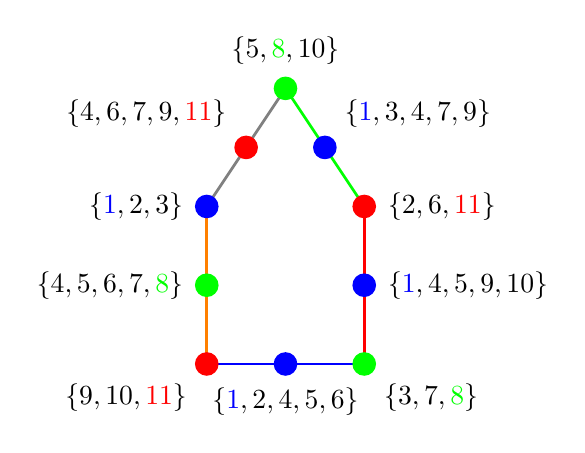
\begin{tikzpicture}  [scale=1]

\tikzstyle{every path}=[line width=1pt]

\newdimen\ms
\ms=0.1cm
\tikzstyle{s1}=[color=red,rectangle,inner sep=3.5]
\tikzstyle{c3}=[circle,inner sep={\ms/8},minimum size=5*\ms]
\tikzstyle{c2}=[circle,inner sep={\ms/8},minimum size=3*\ms]
\tikzstyle{c1}=[circle,inner sep={\ms/8},minimum size=2*\ms]

% Define positions of all observables

\coordinate (a1) at (0,2);
\coordinate (a2) at (0,1);
\coordinate (a3) at (0,0);
\coordinate (a4) at (1,0);
\coordinate (a5) at (2,0);
\coordinate (a6) at (2,1);
\coordinate (a7) at (2,2);
\coordinate (a8) at (1.5,{2+(3.5-2)/2});
\coordinate (a9) at (1,3.5);
\coordinate (a10) at (0.5,{2+(3.5-2)/2});

% draw contexts

\draw [color=orange] (a1) -- (a3);
\draw [color=blue] (a3) -- (a5);
\draw [color=red] (a5) -- (a7);
\draw [color=green] (a7) -- (a9);
\draw [color=gray] (a9) -- (a1);

% draw atoms

\draw (a1) coordinate[c2,fill=blue,label=left:{$\{{\color{blue}1},2,3\}$}];

\draw (a2) coordinate[c2,fill=green,label=left:{$\{ 4,5,6,7,{\color{green}8} \}$}];

\draw (a3) coordinate[c2,fill=red,label=below left:{$\{  9,10,{\color{red}11}\}$}];

\draw (a4) coordinate[c2,fill=blue,label=below:{$\{ {\color{blue}1},2,4,5,6 \}$}];

\draw (a5) coordinate[c2,fill=green,label=below right:{$\{ 3,7,{\color{green}8} \}$}];

\draw (a6) coordinate[c2,fill=blue,label=right:{$\{ {\color{blue}1},4,5,9,10 \}$}];

\draw (a7) coordinate[c2,fill=red,label=right:{$\{ 2,6,{\color{red}11} \}$}];

\draw (a8) coordinate[c2,fill=blue,label=above right:{$\{ {\color{blue}1},3,4,7,9 \}$}];

\draw (a9) coordinate[c2,fill=green,label=above:{$\{ 5,{\color{green}8},10 \}$}];

\draw (a10) coordinate[c2,fill=red,label=above left:{$\{ 4,6,7,9,{\color{red}11} \}$}];

\end{tikzpicture}
\end{center}
\caption{\label{2020-f-chroma-pentagon3}
Coloring scheme of the house/pentagon/pentagram logic from the set of two-valued states.
}
\end{figure}


\subsubsection{``Specker bug'' gadget}

The hypergraph depicted in Fig.~\ref{2020-f-SpeckerBug}
is a minimal~\cite{2018-minimalYIYS} true-implies false gadget introduced by
Kochen and Specker~\cite[Fig.~1, p.~182]{kochen2} (see also ~\cite[Fig.~1, p.~123]{Greechie1974}, among others).
It is a subgraph of $G_{32}$ introduced later in Fig.~\ref{2020-f-GreechieG32}.
Its Travice matrix is
\begin{equation}
T_{ij}=\begin{pmatrix}
{\color{blue}1}& {\color{blue}0}& {\color{blue}0}& {\color{blue}1}& {\color{blue}0} &{\color{blue}1}& {\color{blue}0}& {\color{blue}0}& {\color{blue}1}& {\color{blue}0}& {\color{blue}0}& {\color{blue}0}& {\color{blue}0} \\
1& 0& 0& 0& 1 &0& 0& 1& 0& 1& 0& 0& 0 \\
1& 0& 0& 0& 1 &0& 0& 0& 1& 0& 0& 0& 1 \\
0& 1& 0& 1& 0 &1& 0& 1& 0& 0& 1& 0& 0 \\
0& 1& 0& 1& 0 &1& 0& 0& 1& 0& 0& 1& 0 \\
0& 1& 0& 1& 0 &0& 1& 0& 0& 0& 1& 0& 0 \\
{\color{green}0}& {\color{green}1}& {\color{green}0}& {\color{green}0}& {\color{green}1} &{\color{green}0}& {\color{green}0}& {\color{green}1}& {\color{green}0}& {\color{green}1}& {\color{green}0}& {\color{green}1}& {\color{green}0} \\
0& 1& 0& 0& 1 &0& 0& 1& 0& 0& 1& 0& 1 \\
0& 1& 0& 0& 1 &0& 0& 0& 1& 0& 0& 1& 1 \\
0& 0& 1& 0& 0 &1& 0& 1& 0& 1& 0& 1& 0 \\
0& 0& 1& 0& 0 &1& 0& 1& 0& 0& 1& 0& 1 \\
0& 0& 1& 0& 0 &1& 0& 0& 1& 0& 0& 1& 1 \\
0& 0& 1& 0& 0 &0& 1& 0& 0& 1& 0& 1& 0 \\
{\color{red}0}& {\color{red}0}& {\color{red}1}& {\color{red}0}& {\color{red}0} &{\color{red}0}& {\color{red}1}& {\color{red}0}& {\color{red}0}& {\color{red}0}& {\color{red}1}& {\color{red}0}& {\color{red}1}
\end{pmatrix}
.
\end{equation}

\begin{figure}
\begin{center}
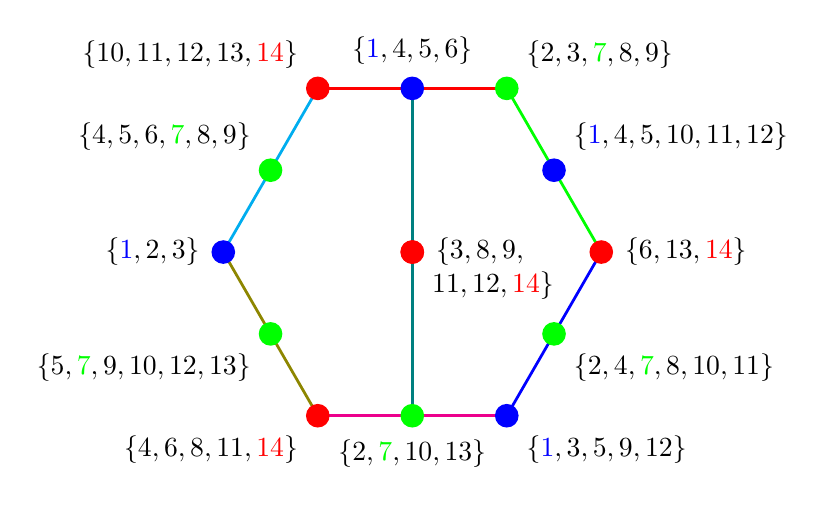
\begin{tikzpicture}  [scale=0.8]

\newdimen\ms
\ms=0.05cm

\tikzstyle{every path}=[line width=1pt]

\tikzstyle{c3}=[circle,inner sep={\ms/8},minimum size=6*\ms]
\tikzstyle{c2}=[circle,inner sep={\ms/8},minimum size=4*\ms]
\tikzstyle{c1}=[circle,inner sep={\ms/8},minimum size=0.8*\ms]

% Radius of regular polygons
\newdimen\R
\R=30mm     % outer circle

%\r= { \R * sqrt(3) }     % inner circle
%\newdimen\r
%\r=    {\R * sqrt(3)/2}       % inner circle

%\newdimen\K
%\K=3cm

% Define positions of all observables
\path
  ({ 180 - 0 * 360 /6}:\R      ) coordinate(1)
  ({ 180 - 30 - 0 * 360 /6}:{\R * sqrt(3)/2}      ) coordinate(2)
  ({ 180 - 1 * 360 /6}:\R   ) coordinate(3)
  ({ 180 - 30 - 1 * 360 /6}:{\R * sqrt(3)/2}   ) coordinate(4)
  ({ 180 - 2 * 360 /6}:\R  ) coordinate(5)
  ({ 180 - 30 - 2 * 360 /6}:{\R * sqrt(3)/2}  ) coordinate(6)
  ({ 180 - 3 * 360 /6}:\R  ) coordinate(7)
  ({ 180 - 30 - 3 * 360 /6}:{\R * sqrt(3)/2}  ) coordinate(8)
  ({ 180 - 4 * 360 /6}:\R     ) coordinate(9)
  ({ 180 - 30 - 4 * 360 /6}:{\R * sqrt(3)/2}     ) coordinate(10)
  ({ 180 - 5 * 360 /6}:\R     ) coordinate(11)
  ({ 180 - 30 - 5 * 360 /6}:{\R * sqrt(3)/2}     ) coordinate(12)
;

% draw contexts

\draw [color=cyan] (1) -- (2) -- (3);
\draw [color=red] (3) -- (4) -- (5);
\draw [color=green] (5) -- (6) -- (7);
\draw [color=blue] (7) -- (8) -- (9);
\draw [color=magenta] (9) -- (10) -- (11);    %
\draw [color=olive] (11) -- (12) -- (1);    %
\draw [color=teal] (4) -- (10)  coordinate[pos=0.5]  (13);

%
%%
%% draw atoms
%%
%
\draw (1) coordinate[c3,fill=blue,label={left: $\{ {\color{blue}1},2,3\} $}];   %
%
\draw (2) coordinate[c3,fill=green,label={above left: $\{ 4,5,6,{\color{green}7},8,9 \}$}];    %
%
\draw (3) coordinate[c3,fill=red,label={above left: $\{10,11,12,13,{\color{red}14} \} $}]; %
%
\draw (4) coordinate[c3,fill=blue,label={above: $\{ {\color{blue}1},4,5,6\}$}];  %
%
\draw (5) coordinate[c3,fill=green,label={above right: $\{ 2,3,{\color{green}7},8,9\} $}];  %
%
\draw (6) coordinate[c3,fill=blue,label={above right: $\{ {\color{blue}1},4,5,10,11,12\} $}];
%
\draw (7) coordinate[c3,fill=red,label={right: $\{ 6,13,{\color{red}14}\}$}];  %
%
\draw (8) coordinate[c3,fill=green,label={below right: $\{ 2,4,{\color{green}7},8,10,11\}$}];  %
%
\draw (9) coordinate[c3,fill=blue,label={below right: $\{ {\color{blue}1},3,5,9,12\}$}];
%
\draw (10) coordinate[c3,fill=green,label={below: $\{ 2,{\color{green}7},10,13\}$}];  %
%
\draw (11) coordinate[c3,fill=red,label={below left: $\{ 4,6,8,11,{\color{red}14}\}$}];  %
%
\draw (12) coordinate[c3,fill=green,label={below left: $\{ 5,{\color{green}7},9,10,12,13\}$}];
%
%
\draw (13) coordinate[c3,fill=red,label={right: $\{3,8,9,$}];  %
\draw (13) coordinate[c3,fill=red,label={below right: $11,12,{\color{red}14}\}$}];  %
%
\end{tikzpicture}
\end{center}
\caption{\label{2020-f-SpeckerBug}
Coloring scheme of the ``Specker bug'' gadget~\cite{kochen2,Greechie1974} from two-valued states.
The set theoretic representation is in terms of
the canonical partition logic as an equipartitioning of the set $\{1,2,\ldots,14\}$
obtained from all 14 two-valued states on this gadget.
}
\end{figure}

\section{Inherited chromatic properties}

\subsection{Color-(in)separability of nonadjacent atoms}

An intertwined combo of Specker bugs -- Kochen \& Specker's $\Gamma_3$~\cite{kochen1} -- is still colorable because the two bugs therein ``inherit''
the colorings of the single bugs. Yet, any set of such colorings is no longer {\em separable} in that two nonadjacent (``complementary'') atoms
allow different colors.

\subsection{Colorings from non-unital set of two-valued states}
In a similar way, non-unital sets of two-valued states ``fix'' the variety of colorings by allowing only a single color at certain atoms.

\subsection{Counterexamples}

\subsubsection{Greechie's $G_{32}$}

It is quite straightforward to demonstrate that the logic $G_{32}$ introduced by Greechie~\cite[Fig.~6, p.~121]{greechie:71}
(see also Refs.~\cite{Holland1975,Bennett-MC-1970,Greechie1974,Greechie-Suppes1976})
whose hypergraph is depicted in Fig.~\ref{2020-f-GreechieG32} has a chromatic number larger than three;
and, in particular, cannot be colored by two-valued states.
Consider the set of all six two-valued states which can be tabulated by the Travis matrix
\begin{equation}
T_{ij}=\begin{pmatrix}
1&0&0&1&0&1&0&0&1&0&0&0&0&0&1\\
1&0&0&0&1&0&0&1&0&1&0&0&0&1&0\\
0&1&0&1&0&0&1&0&0&0&1&0&0&1&0\\
0&1&0&0&1&0&0&0&1&0&0&1&1&0&0\\
0&0&1&0&0&1&0&1&0&0&1&0&1&0&0\\
0&0&1&0&0&0&1&0&0&1&0&1&0&0&1
\end{pmatrix}
.
\end{equation}
There is no way how three of these six row vectors add up to
a vector whose components are all one; that is,
$
\begin{pmatrix}
1,1,1,1,1,1,1,1,1,1,1,1,1,1,1
\end{pmatrix}
$.
``Completing'' the partition logic and ``extending''
$G_{32}$ by adding five more contexts
$\{\{1, 2\}, \{3, 6\}, \{4, 5\}\}$,
$\{\{1, 4\}, \{2, 3\}, \{5, 6\}\}$,
$\{\{1, 3\}, \{2, 5\}, \{4, 6\}\}$,
$\{\{1, 5\}, \{2, 6\}, \{3, 4\}\}$, and
$\{\{1, 6\}, \{2, 4\}, \{3, 5\}\}$
does not change the set of two-valued states and thus the Travis matrix.


Another way of seing this is to associate a color to, say, the first state.
As a consequence, all other states, namely states number
$2$,
$3$,
$4$,
$5$, and
$6$, need to be eliminated,
leaving no state which can be associated with
another color.

\begin{figure}
\begin{center}
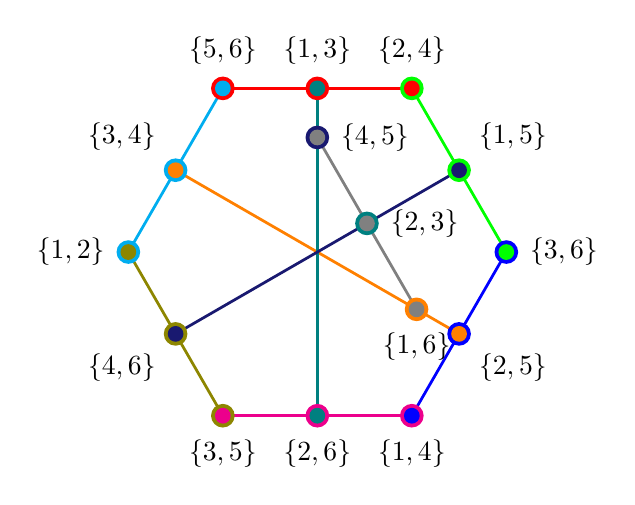
\begin{tikzpicture}  [scale=0.8]

\newdimen\ms
\ms=0.05cm

\tikzstyle{every path}=[line width=1pt]

\tikzstyle{c3}=[circle,inner sep={\ms/8},minimum size=6*\ms]
\tikzstyle{c2}=[circle,inner sep={\ms/8},minimum size=4*\ms]
\tikzstyle{c1}=[circle,inner sep={\ms/8},minimum size=0.8*\ms]

% Radius of regular polygons
\newdimen\R
\R=30mm     % outer circle

%\r= { \R * sqrt(3) }     % inner circle
%\newdimen\r
%\r=    {\R * sqrt(3)/2}       % inner circle

%\newdimen\K
%\K=3cm

% Define positions of all observables
\path
  ({ 180 - 0 * 360 /6}:\R      ) coordinate(1)
  ({ 180 - 30 - 0 * 360 /6}:{\R * sqrt(3)/2}      ) coordinate(2)
  ({ 180 - 1 * 360 /6}:\R   ) coordinate(3)
  ({ 180 - 30 - 1 * 360 /6}:{\R * sqrt(3)/2}   ) coordinate(4)
  ({ 180 - 2 * 360 /6}:\R  ) coordinate(5)
  ({ 180 - 30 - 2 * 360 /6}:{\R * sqrt(3)/2}  ) coordinate(6)
  ({ 180 - 3 * 360 /6}:\R  ) coordinate(7)
  ({ 180 - 30 - 3 * 360 /6}:{\R * sqrt(3)/2}  ) coordinate(8)
  ({ 180 - 4 * 360 /6}:\R     ) coordinate(9)
  ({ 180 - 30 - 4 * 360 /6}:{\R * sqrt(3)/2}     ) coordinate(10)
  ({ 180 - 5 * 360 /6}:\R     ) coordinate(11)
  ({ 180 - 30 - 5 * 360 /6}:{\R * sqrt(3)/2}     ) coordinate(12)
;

% draw contexts

\draw [color=cyan] (1) -- (2) -- (3);
\draw [color=red] (3) -- (4) -- (5);
\draw [color=green] (5) -- (6) -- (7);
\draw [color=blue] (7) -- (8) -- (9);
\draw [color=magenta] (9) -- (10) -- (11);    %
\draw [color=olive] (11) -- (12) -- (1);    %
\draw [color=orange] (2) -- (8)  coordinate[pos=0.85]  (15);
\draw [color=teal] (4) -- (10)  coordinate[pos=0.15]  (13);
\draw [color=MidnightBlue] (6) -- (12)  coordinate[pos=0.325]  (14);
\draw [color=gray] (13) --(15);

%
%%
%% draw atoms
%%
%
\draw (1) coordinate[c3,fill=cyan,label={left: $\{ 1,2\} $}];   %
\draw (1) coordinate[c2,fill=olive];  %
%
\draw (2) coordinate[c3,fill=cyan,label={above left: $\{ 3,4\}$}];    %
\draw (2) coordinate[c2,fill=orange];    %
%
\draw (3) coordinate[c3,fill=red,label={above: $\{ 5,6\} $}]; %
\draw (3) coordinate[c2,fill=cyan];  %
%
\draw (4) coordinate[c3,fill=red,label={above: $\{ 1,3\}$}];  %
\draw (4) coordinate[c2,fill=teal];  %
%
\draw (5) coordinate[c3,fill=green,label={above: $\{ 2,4\} $}];  %
\draw (5) coordinate[c2,fill=red];  %
%
\draw (6) coordinate[c3,fill=green,label={above right: $\{ 1,5\} $}];
\draw (6) coordinate[c2,fill=MidnightBlue];
%
\draw (7) coordinate[c3,fill=blue,label={right: $\{ 3,6\}$}];  %
\draw (7) coordinate[c2,fill=green];  %
%
\draw (8) coordinate[c3,fill=blue,label={below right: $\{ 2,5\}$}];  %
\draw (8) coordinate[c2,fill=orange];  %
%
\draw (9) coordinate[c3,fill=magenta,label={below: $\{ 1,4\}$}];
\draw (9) coordinate[c2,fill=blue];  %
%
\draw (10) coordinate[c3,fill=magenta,label={below: $\{ 2,6\}$}];  %
\draw (10) coordinate[c2,fill=teal];  %
%
\draw (11) coordinate[c3,fill=olive,label={below: $\{ 3,5\}$}];  %
\draw (11) coordinate[c2,fill=magenta];  %
%
\draw (12) coordinate[c3,fill=olive,label={below left: $\{ 4,6\}$}];
\draw (12) coordinate[c2,fill=MidnightBlue];
%
\draw (13) coordinate[c3,fill=MidnightBlue,label={right: $\{ 4,5\}$}];  %
\draw (13) coordinate[c2,fill=gray];  %
%
\draw (14) coordinate[c3,fill=teal,label=0:{$\{ 2,3\}$}];  %
\draw (14) coordinate[c2,fill=gray];  %
%
\draw (15) coordinate[c3,fill=orange,label={below: $\{1,6\}$}];  %
\draw (15) coordinate[c2,fill=gray];  %
%
\end{tikzpicture}
\end{center}
\caption{\label{2020-f-GreechieG32}
Greechie diagram of $G_{32}$ introduced by Greechie~\cite[Fig.~6, p.~121]{greechie:71}.
The overlaid set theoretic representation is in terms of
the canonical partition logic as an equipartitioning of the set $\{1,2,3,4,5,6\}$
obtained from all 6 two-valued states on $G_{32}$.
}
\end{figure}

\begin{acknowledgments}
The author acknowledges the support by the Austrian Science Fund (FWF): project I 4579-N and the Czech Science Foundation (GA\v CR): project 20-09869L.

The author declares no conflict of interest.

I kindly acknowledge enlightening discussions with Adan Cabello, Jos\'{e} R. Portillo, and Mohammad Hadi Shekarriz.
I am grateful to Josef Tkadlec for providing a {\em Pascal} program
which computes and analyses the set of two-valued states of collections of contexts.
All misconceptions and errors are mine.
\end{acknowledgments}



% MDPI \funding{The author acknowledges the support by the Austrian Science Fund (FWF): project I 4579-N and the Czech Science Foundation (GA\v CR): project 20-09869L.}

%%%%%%%%%%%%%%%%%%%%%%%%%%%%%%%%%%%%%%%
% MDPI \acknowledgments{I kindly acknowledge enlightening discussions with Adan Cabello, Jos\'{e} R. Portillo, and Mohammad Hadi Shekarriz.
% MDPI I am grateful to Josef Tkadlec for providing a {\em Pascal} program
% MDPI which computes and analyses the set of two-valued states of collections of contexts.
% MDPI All misconceptions and errors are mine.
% MDPI The author declares no conflict of interest.
% MDPI }

%%%%%%%%%%%%%%%%%%%%%%%%%%%%%%%%%%%%%%%
% MDPI \conflictsofinterest{The author declares no conflict of interest.}


%%%%%%%%%%%%%%%%%%%%%%%%%%%%%%%%%%%%%%%
% MDPI \reftitle{References}

% Please provide either the correct journal abbreviation (e.g. according to the “List of Title Word Abbreviations” http://www.issn.org/services/online-services/access-to-the-ltwa/) or the full name of the journal.
% Citations and References in Supplementary files are permitted provided that they also appear in the reference list here.

%=====================================
% References, variant A: external bibliography
%=====================================
%\externalbibliography{yes}

 \bibliography{svozil}
 \bibliographystyle{apsrev}



%%%%%%%%%%%%%%%%%%%%%%%%%%%%%%%%%%%%%%%

\end{document}

%%%%%%%%%%%%%%%%%%%%%%%%%%%%%%%%%%%%%%%%%%%%%%%%%%%%%%%%%%%%%%%%%%%%%%%%%%%%%%%%%%%%%%%%%%%%%%%%%%%%%%%%%%%%%%%%%%%%%%%%%%%%%%%%%%%%%%%

house-pentagon-pentagram
10 atoms
 5 blocks
 0 proper subsets of blocks
 3   1  2  3
 3   3  4  5
 3   5  6  7
 3   7  8  9
 3   9 10  1
11 2-valued evaluations of atoms:
1 0 0 1 0 1 0 1 0 0
1 0 0 1 0 0 1 0 0 0
1 0 0 0 1 0 0 1 0 0
0 1 0 1 0 1 0 1 0 1
0 1 0 1 0 1 0 0 1 0
0 1 0 1 0 0 1 0 0 1
0 1 0 0 1 0 0 1 0 1
0 1 0 0 1 0 0 0 1 0
0 0 1 0 0 1 0 1 0 1
0 0 1 0 0 1 0 0 1 0
0 0 1 0 0 0 1 0 0 1

set of 2-valued evaluations of atoms:
nonempty: yes
unital: yes
separating atoms: yes
separating: yes
1s on nonorthogonal atoms (=OD if no noncomplete block): yes
order determining: yes

%%%%%%%%%%%%%%%%%%%%%%%%%%%%%%%%%%%%%%%%%%%%%%%%%%%%%%%%%%%%%%%%%%%%%%%%%%%%%%%%%%%%%%%%%%%%%%%%%%%%%%%%%%%%%%%%%%%%%%%%%%%%%%%%%%%%%%%

Specker bug
13 atoms
 7 blocks
 0 proper subsets of blocks
 3   1  2  3
 3   3  4  5
 3   5  6  7
 3   7  8  9
 3   9 10 11
 3  11 12  1
 3   4 10 13
14 2-valued evaluations of atoms:
1 0 0 1 0 1 0 0 1 0 0 0 0
1 0 0 0 1 0 0 1 0 1 0 0 0
1 0 0 0 1 0 0 0 1 0 0 0 1
0 1 0 1 0 1 0 1 0 0 1 0 0
0 1 0 1 0 1 0 0 1 0 0 1 0
0 1 0 1 0 0 1 0 0 0 1 0 0
0 1 0 0 1 0 0 1 0 1 0 1 0
0 1 0 0 1 0 0 1 0 0 1 0 1
0 1 0 0 1 0 0 0 1 0 0 1 1
0 0 1 0 0 1 0 1 0 1 0 1 0
0 0 1 0 0 1 0 1 0 0 1 0 1
0 0 1 0 0 1 0 0 1 0 0 1 1
0 0 1 0 0 0 1 0 0 1 0 1 0
0 0 1 0 0 0 1 0 0 0 1 0 1

set of 2-valued evaluations of atoms:
nonempty: yes
unital: yes
separating atoms: yes
separating: yes
1s on nonorthogonal atoms (=OD if no noncomplete block): no for atoms
 1/7
1s on nonorthogonal atoms (=1D if no noncomplete block): yes
order determining: no for sets of atoms (ordered elements?)
 7/2+3
 1/5+6

%%%%%%%%%%%%%%%%%%%%%%%%%%%%%%%%%%%%%%%%%%%%%%%%%%%%%%%%%%%%%%%%%%%%%%%%%%%%%%%%%%%%%%%%%%%%%%%%%%%%%%%%%%%%%%%%%%%%%%%%%%%%%%%%%%%%%%%


Greechie G32 bug
15 atoms
10 blocks
 0 proper subsets of blocks
 3   1  2  3
 3   3  4  5
 3   5  6  7
 3   7  8  9
 3   9 10 11
 3  11 12  1
 3   4 10 13
 3   6 12 14
 3   8  2 15
 3  13 14 15
6 2-valued evaluations of atoms:
1 0 0 1 0 1 0 0 1 0 0 0 0 0 1
1 0 0 0 1 0 0 1 0 1 0 0 0 1 0
0 1 0 1 0 0 1 0 0 0 1 0 0 1 0
0 1 0 0 1 0 0 0 1 0 0 1 1 0 0
0 0 1 0 0 1 0 1 0 0 1 0 1 0 0
0 0 1 0 0 0 1 0 0 1 0 1 0 0 1

set of 2-valued evaluations of atoms:
nonempty: yes
unital: yes
separating atoms: yes
separating: yes
1s on nonorthogonal atoms (=OD if no noncomplete block): no for atoms
 1/7 1/13 2/6 2/10 3/9 3/14 4/8 4/12 5/11 5/15 6/10 7/13 8/12 9/14 11/15
order determining: no for sets of atoms (ordered elements?)
 3/7+8
 3/6+12
 2/5+7
 2/9+11
 7/2+3
 13/2+3
 1/5+6
 1/4+10
 6/1+3
 10/1+3
 9/1+2
 14/1+2
 5/9+10
 5/2+8
 4/7+9
 4/1+11
 8/3+5
 12/3+5
 11/3+4
 15/3+4
 7/4+10
 6/9+11
 10/5+7
 13/5+6
 9/6+12
 8/1+11
 12/7+9
 14/7+8
 11/2+8
 15/9+10


%%%%%%%%%%%%%%%%%%%%%%%%%%%%%%%%%%%%%%%%%%%%%%%%%%%%%%%%%%%%%%%%%%%%%%%%%%%%%%%%%%%%%%%%%%%%%%%%%%%%%%%%%%%%%%%%%%%%%%%%%%%%%%%%%%%%%%%

KSetPartitions[{1, 2, 3, 4, 5, 6}, 3] // MatrixForm

{
 {{1, 2}, {3, 4}, {5, 6}}
 {{1, 2}, {3, 6}, {4, 5}},
 {{1, 2}, {3, 5}, {4, 6}},
 {{1, 4}, {2, 3}, {5, 6}},
 {{1, 3}, {2, 4}, {5, 6}},
 {{1, 6}, {2, 3}, {4, 5}},
 {{1, 3}, {2, 6}, {4, 5}},
 {{1, 5}, {2, 3}, {4, 6}},
 {{1, 3}, {2, 5}, {4, 6}},
 {{1, 6}, {2, 5}, {3, 4}},
 {{1, 5}, {2, 6}, {3, 4}},
 {{1, 6}, {2, 4}, {3, 5}},
 {{1, 4}, {2, 6}, {3, 5}},
 {{1, 5}, {2, 4}, {3, 6}},
 {{1, 4}, {2, 5}, {3, 6}}
}

KSetPartitions[{1, 2, 3, 4, 5, 6}, 3] // MatrixForm

{
                {{1, 2}, {3, 4}, {5, 6}},
 {{1, 2}, {3, 6}, {4, 5}},
                {{1, 2}, {3, 5}, {4, 6}},
 {{1, 4}, {2, 3}, {5, 6}},
                {{1, 3}, {2, 4}, {5, 6}},
                {{1, 6}, {2, 3}, {4, 5}},
                {{1, 3}, {2, 6}, {4, 5}},
                {{1, 5}, {2, 3}, {4, 6}},
 {{1, 3}, {2, 5}, {4, 6}},
                {{1, 6}, {2, 5}, {3, 4}},
 {{1, 5}, {2, 6}, {3, 4}},
 {{1, 6}, {2, 4}, {3, 5}},
                {{1, 4}, {2, 6}, {3, 5}},
                {{1, 5}, {2, 4}, {3, 6}},
                {{1, 4}, {2, 5}, {3, 6}}
}


Greechie G32 bug  extended
15 atoms
15 blocks
 0 proper subsets of blocks
 3   1  2  3
 3   3  4  5
 3   5  6  7
 3   7  8  9
 3   9 10 11
 3  11 12  1
 3   4 10 13
 3   6 12 14
 3   8  2 15
 3  13 14 15
 3   1  7 13
 3   4  8 12
 3   2  6 10
 3   3  9 14
 3   5 11 15
6 2-valued evaluations of atoms:
1 0 0 1 0 1 0 0 1 0 0 0 0 0 1
1 0 0 0 1 0 0 1 0 1 0 0 0 1 0
0 1 0 1 0 0 1 0 0 0 1 0 0 1 0
0 1 0 0 1 0 0 0 1 0 0 1 1 0 0
0 0 1 0 0 1 0 1 0 0 1 0 1 0 0
0 0 1 0 0 0 1 0 0 1 0 1 0 0 1

set of 2-valued evaluations of atoms:
nonempty: yes
unital: yes
separating atoms: yes
separating: yes
1s on nonorthogonal atoms (=OD if no noncomplete block): yes
order determining: yes
